\chapter{Аналитический раздел}

В данном разделе представлены основные теоритические сведения о двоичных деревьях и хеш-таблицах, а также описано техническое задание.

\section{Основные теоритические сведения}

Ниже представлены основные теоритические сведения, касаемые таких структур данных как двоичное дерево поиска, сбалансированное двоичное дерево поиска и хеш-таблица.

\subsection{Двоичное дерево поиска}

Дерево  –  это  нелинейная  структура  данных,  используемая  для  представления 
иерархических связей, имеющих отношение «один ко многим». 

К  основным  операциям,  выполняемым  с  различными  структурами 
данных,  можно  отнести  поиск  среди  набора  данных.  Один  из  широко 
используемых  для  этого  методов  —  построение  двоичного  дерева  поиска, которое ускоряет и упрощает задачу поиска данных в определенном  наборе  информации,  структурирует  заданную  информацию  для 
более  эффективного  ее  дальнейшего  использования,  а  при  отсутствии 
необходимой информации возвращает указатель на пустой элемент \cite{virt}. 

Дерево двоичного поиска –  это такое дерево, в котором все левые потомки моложе 
предка,  а  все  правые  – старше.  Это  свойство  называется  характеристическим 
свойством дерева двоичного поиска и выполняется для любого узла, включая корень. 
С учетом этого свойства поиск узла в двоичном дереве поиска можно осуществить, 
двигаясь от корня в левое или правое поддерево в зависимости от значения ключа 
поддерева. 

\subsection{Сбалансированное двоичное дерево поиска}

Если  при  построении  дерева  поочередно  располагать  узлы  слева  и  справа,  то 
получится дерево, у которого число вершин в левом и правом поддеревьях отличается 
не более чем на единицу. Такое дерево называется идеально сбалансированным.

$N$ элементов можно организовать в бинарное дерево с высотой не более $log_2(N)$, поэтому для поиска среди $N$ элементов может потребоваться не больше $log_2(N)$ сравнений, если дерево идеально сбалансировано. 

Адельсон-Вельский  и  Ландис  сформулировали  менее  жесткий  критерий 
сбалансированности таким образом: двоичное дерево называется сбалансированным, 
если  у  каждого  узла  дерева  высота  двух  поддеревьев  отличается  не  более  чем  на 
единицу. Такое дерево называется АВЛ-деревом.

Использование  этого  критерия  приводит  к  легко  выполняемой  балансировке. 
При  этом  средняя  длина  поиска  остается  практически  такой  же,  как  и  у  идеально 
сбалансированного дерева.  
При  включении  узла  в  сбалансированное  дерево  возможны  3  случая: 
(рассматриваем включение в левое поддерево):

\begin{enumerate}
    \item Левое  и  правое  поддеревья  становятся  неравной  высоты,  но  критерий 
    сбалансированности не нарушается.
    \item Левое  и  правое  поддерево  приобретают  равную  высоту  и,  таким  образом, 
    сбалансированность даже улучшается.
    \item Критерий сбалансированности нарушается, и дерево надо перестраивать.
\end{enumerate}

Алгоритм включения и балансировки существенно зависит от способа хранения 
информации  о  сбалансированности  дерева.  Одно  из  решений  –  хранить  в  каждой 
вершине показатель ее сбалансированности. В этом случае сбалансированность будет 
определяться как разность между высотой правого и левого поддеревьев

Отсюда следует, что дерево – это  
более подходящая структура для организации поиска, чем, например, линейный список.

\subsection{Хеш-таблицы}

Массив, заполненный в порядке, определенным хеш-функцией, называется \textit{хеш-таблицей}. Хеш-функции позволяют по значению ключа определять сразу индекс элемента массива, в котором хранится информация. Минимальная трудоемкость поиска в хеш-таблице равна $O(1)$.

Принято считать, что хорошей является такая функция, которая удовлетворяет 
следующим условиям: 

\begin{itemize}[$\bullet$]
    \item функция должна быть простой с вычислительной точки зрения;
    \item функция должна распределять ключи в хеш-таблице наиболее равномерно.
\end{itemize}

Сформулируем понятие коллизии следующим образом. Пусть есть хеш-функция $H$. Если найдены две различных строки $U,~W$  со свойством $H(U) 
= H(W)$, то обнаружена коллизия при хешировании с помощью функции $H$ \cite{hash}.

Существует  несколько  возможных  вариантов  разрешения  коллизий,  которые имеют свои достоинства и недостатки.

\textbf{Первый метод:} внешнее (открытое) хеширование (метод цепочек). 

В случае, когда элемент таблицы с индексом, который вернула хеш-функция, 
уже  занят,  к  нему  присоединяется  связный  список.  Таким  образом,  если  для 
нескольких  различных  значений  ключа  возвращается  одинаковое  значение  хеш-функции,  то  по  этому  адресу  находится  указатель  на  связанный  список,  который 
содержит все значения. Поиск в этом списке осуществляется простым перебором, так 
как при грамотном выборе хеш-функции любой из списков оказывается достаточно 
коротким.

\textbf{Второй метод:} внутреннее (закрытое) хеширование (открытая адресация).

Состоит в том, чтобы полностью 
отказаться от ссылок. В этом случае, если ячейка с вычисленным индексом занята, то 
можно просто просматривать следующие записи таблицы по порядку (с шагом 1), до 
тех пор, пока не будет найден ключ K или пустая позиция в таблице. При этом, если 
индекс следующего просматриваемого элемента определяется добавлением какого-то 
постоянного  шага  (от  1  до  n),  то  данный  способ  разрешения  коллизий  называется 
линейной адресацией. Для вычисления шага можно также применить формулу:

\begin{equation}
    h = h + a^2
\end{equation}

где  $a$  – это  номер  попытки  поиска  ключа.  Этот  вид  адресации  называется 
квадратичной или произвольной адресацией. 

При любом методе разрешения коллизий необходимо ограничить длину поиска 
элемента.  Если  для  поиска  элемента  необходимо  более  3–4  сравнений,  то 
эффективность  использования  такой  хеш-таблицы  пропадает  и  ее  следует 
реструктуризировать  (т.е.  найти  другую  хеш-функцию),  чтобы  минимизировать 
количество сравнений для поиска элемента  

\section{Техническое задание}

\subsection{Общее задание}

Построить дерево в соответствии с заданным вариантом задания. Вывести его 
на  экран  в  виде  дерева.  Реализовать  основные  операции  работы  с  деревом:  обход 
дерева, включение, исключение и поиск узлов. Сравнить эффективность алгоритмов 
сортировки  и  поиска  в  зависимости  от  высоты  дерева  и  степени  его  ветвления. 
Построить  хеш-таблицу  по  указанным  данным.  Вывести  на  экран  деревья  и  хеш-таблицу.  Сравнить  эффективность  поиска  в  двоичном  дереве  поиска,  в 
сбалансированном  дереве  поиска  и  в  хеш-таблице.  Вывести  на  экран  измененные 
структуры.  Подсчитать  среднее  количество  сравнений  для  поиска  данных  в 
указанных  структурах.  Произвести  реструктуризацию  хеш-таблицы,  если  среднее 
количество  сравнений  больше  указанного.  Оценить  эффективность  использования 
этих структур (по времени и памяти) для поставленной задачи.

\subsection{Задание варианта}

\textbf{Вариант 4:}

В текстовом файле содержатся целые числа. Построить ДДП из чисел файла. 
Вывести его на экран в виде дерева. Сбалансировать полученное дерево и 
вывести его на экран. Построить хеш-таблицу из чисел файла. Использовать 
закрытое  хеширование  для  устранения  коллизий.  Осуществить  удаление 
введенного целого числа в ДДП, в сбалансированном дерево, в хеш-таблице и в 
файле. Сравнить время удаления, объем памяти и количество сравнений при 
использовании различных (4-х) структур данных. Если количество сравнений в 
хеш-таблице  больше  указанного,  то  произвести  реструктуризацию  таблицы, 
выбрав другую функцию.

\chapter{Конструкторский раздел}

В данном разделе представлена информация об используемых структурах данных, а также приведены схемы реализуемых алгоритмов.

\section{Функции хеширования}

В рамках данной лабораторной работы реализованы две функции хеширования, реализованные по следующим схемам:

\begin{itemize}[$\bullet$]
    \item метод деления;
    \item мультипликативная схема.
\end{itemize}

\subsection{Метод деления}

Метод деления основан на простой операции -- взятии остатка от деления. Для данного метода возьмем остаток от деления на M:

\begin{equation}
    h(K) = K~mod~M
\end{equation}

\subsection{Мультипликативная схема}

Ниже представлена функция хеширования для мультипликативной формы.

Пусть $\omega$ --- размер машинного слова. Метод состоит в выборе некоторой целой константы $A$, взаимно простой с $\omega$, после чего можно положить: 

\begin{equation}
    h(K) = \lfloor M\left(\left(\frac{A}{\omega}K\right)~mod~1\right) \rfloor
\end{equation}

Мультипликативная схема хеширования реализуется на основе хеширования Фиббоначи: $\frac{A}{\omega}$ приблизительно равно золотому сечению $\phi = \frac{\sqrt{5} - 1}{2} \approx 0.6180339887$.

\section{Разрешение коллизий}

Для разрешения коллизий используется схема адресации, известная как линейное исследование, которая использует циклическую последовательность проверок:

\begin{equation}
    h(K),~ h(K)+1,~ \dots,~ M-2,~ M-1,~0,~1,~ \dots,~ h(K)-1
\end{equation}

\section{Схемы алгоритмов}

Ниже, на рисунке \ref{algo:balance}, представлен алгоритм балансировки для поддерева двоичного дерева поиска. Для полной балансировки необходимо рекурсивно применить этот алгоритм ко всем узлам дерева.

\begin{figure}
    \centering
    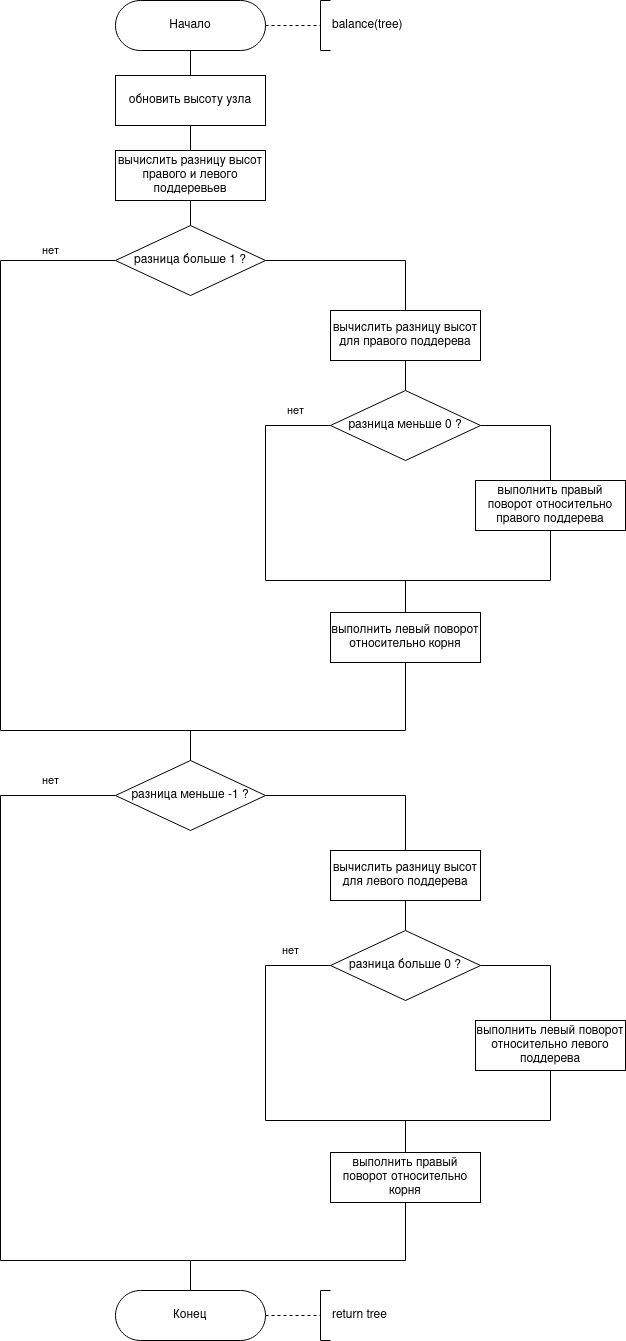
\includegraphics[width=0.6\linewidth]{balance.png}
    \caption{Алгоритм балансировки}
    \label{algo:balance}
\end{figure}

\clearpage

\section{Структуры данных}

Ниже, на листинге \ref{struct:avl}, представлена структура АВЛ-дерева.

\begin{lstlisting}[language=C,caption=Структура АВЛ-дерева,label=struct:avl]
typedef struct avl_node
{
    data_t key;
    uint8_t height;

    struct avl_node *left;
    struct avl_node *right;
} node_t;
\end{lstlisting}

Ниже, на листинге \ref{struct:hash}, представлена структура хеш-таблицы.

\begin{lstlisting}[language=C,caption=Структура хеш-таблицы,label=struct:hash]
typedef struct
{
    data_t key;
    bool has_value;
    size_t cmp_count;
} hash_data_t;

typedef struct
{
    size_t size;
    size_t step;
    hash_data_t *data;
    hf_t func;
} hash_table_t;
\end{lstlisting}

\clearpage

\section{Реализуемые функции}

Ниже, на листинге \ref{func:trees}, представлены функции для работы с двоичными деревьями поиска и АВЛ-деревьями.

\begin{lstlisting}[language=C,caption=Функции для работы с деревьями,label=func:trees]
// ================================================================================
// ДДП
// ================================================================================

/**
    * @brief Ввод бинарного дерева поиска (не сбалансированного)
    * 
    * @param filename имя файла, содержащего целые числа
    * @return node_t* (указатель на корень дерева)
    */
node_t *bst_input(const char *filename);

/**
    * @brief Вывод бинарного дерева поиска в графическом виде
    * 
    * @param root корень ДДП
    */
void bst_output(const node_t *root, const char *graphname);

/**
    * @brief Освобождение памяти из-под бинарного дерева
    * 
    * @param root корень ДДП 
    */
void bst_destroy(node_t *root);

/**
    * @brief Поиск элемента в ДДП
    * 
    * @param root корень ДДП
    * @param key искомый элемент
    * @return node_t* (искомый узел)
    */
const node_t *bst_search(const node_t *root, data_t key, size_t *cmp_count);

/**
    * @brief Удаление элемента из дДП
    * 
    * @param root корень ДДП
    * @param key удаляемый элемент
    * @return node_t* (искомый узел)
    */
node_t *bst_remove(node_t *root, data_t key, size_t *cmp_count);

double bst_get_mean_cmp_count(const node_t *root);

/**
    * @brief Вычисляет размер занимаемой деревом памяти
    */
size_t bst_sizeof(const node_t *root);

/**
    * @brief Преобразование ДДП в АВЛ-дерево
    * 
    * @param node узел дерева
    * @return node_t* (корень сбалансированного АВЛ дерева)
    */
node_t *bst_to_avl(node_t *node);

// ====================================================================================
// АВЛ-деревья
// ====================================================================================

/**
    * @brief Выделяет память под узел дерева
    * 
    * @param key значение узла
    * @return node_t* (указатель на выделенную область памяти)
    */
node_t *node_init(data_t key);

/**
    * @brief Обёртка поля height, которая может работать с нулевыми указателями
    * 
    * @param node узел дерева
    * @return uint8_t (высота поддерева)
    */
uint8_t height(node_t *node);

/**
    * @brief Вычисление показателя балансировки узла
    * 
    * @param node узел дерева, балансировка которого вычисляется
    * @return int (показатель балансировки узла)
    */
int bfactor(node_t *node);

/**
    * @brief Восстанавливает корректное значения поля height
    * 
    * @param node узел, высота которого исправляется
    */
void fix_height(node_t *node);

/**
    * @brief Балансировка при вставке в отбалансированное дерево
    * 
    * @param node узел дерева
    * @return node_t* (корень сбалансированного дерева)
    */
node_t *balance(node_t *node);

/**
    * @brief Вставить значение в дерево, сохранив балансировку
    * 
    * @param root корень дерева
    * @param key значение узла
    * @return node_t* (корень сбалансированного дерева)
    */
node_t *avl_insert(node_t *root, data_t key);

/**
    * @brief Удаления ключа key из данного дерева
    * 
    * @param root корень дерева
    * @param key ключ, подлежащий удалению
    * @param[out] cmp_count количество сравнений
    * @return node_t* (указатель на новое дерево)
    */
node_t *avl_remove(node_t *root, data_t key, size_t *cmp_count);

\end{lstlisting}

Ниже, на листинге \ref{func:hash}, представлены функции для работы с хеш-таблицами.

\begin{lstlisting}[language=C,caption=Функции для работы с хеш-таблицами,label=func:hash]
/**
* @brief Нулевая хеш-таблица
* 
* @return hash_table_t 
*/
hash_table_t hash_null(void);

/**
* @brief Выделение памяти под хеш-таблицу
* 
* @param size размер хеш-таблицы
* @param step шаг для устранения коллизий
* @param func хеш-функция
* @return hash_table_t 
*/
hash_table_t hash_init(size_t size, size_t step, hf_t func);

/**
* @brief Освобождение памяти из-под хеш-таблицы
* 
* @param table хеш-таблица
*/
void hash_destroy(hash_table_t *table);

/**
* @brief Ввод хеш-таблицы
* 
* @param table хеш-таблицы
* @param size максимальный размер хеш-таблицы
* @param filename имя входного файла
* @return int 
*/
int hash_input(hash_table_t *table, size_t size, const char *filename);

/**
* @brief Вывод хеш-таблицы
* 
* @param table хеш-таблица
*/
void hash_output(const hash_table_t *table);

/**
* @brief Поиск в хеш-таблице
* 
* @param table хеш-таблица
* @param data искомый ключ
* @return true 
* @return false 
*/
bool hash_find(hash_table_t *table, data_t data);

/**
* @brief Вставка в хеш-таблицу
* 
* @param table хеш-таблица
* @param data ключ
* @return int 
*/
int hash_insert(hash_table_t *table, data_t data);

/**
* @brief Удаление из хеш-таблицы
* 
* @param table хеш-таблица
* @param data удаляемый ключ
* @param cmp_count максимальное число сравнений
* @return int 
*/
int hash_remove(hash_table_t *table, data_t data, size_t *cmp_count);

/**
* @brief Вычисление среднего числа сравнений
* 
* @param table хеш-таблица
* @return double 
*/
double hash_get_mean_cmp_count(const hash_table_t *table);

/**
* @brief Вычисление максимального числа сравнений
* 
* @param table хеш-таблица
* @return size_t 
*/
size_t hash_get_max_cmp_count(const hash_table_t *table);

/**
* @brief Размер занимаемый под хеш-таблицу памяти
* 
* @param table хеш-таблица
* @return size_t 
*/
size_t hash_sizeof(const hash_table_t *table);

/**
* @brief Реструктуризация хеш-таблицы
* 
* @param table хеш-таблица
* @return int 
*/
int hash_restruct(hash_table_t *table);

/**
* @brief Хеш-функция на основе деления
* 
* @param data данные, подлежащие хешированию
* @param table_size размер хеш-таблицы
* @return size_t 
*/
size_t hasher1(data_t data, size_t table_size);

/**
* @brief Хеш-функция на основе хеширования Фиббоначи (мультипликативная форма)
* 
* @param data данные, подлежащие хешированию
* @param table_size размер хеш-таблицы
* @return size_t 
*/
size_t hasher2(data_t data, size_t table_size);
\end{lstlisting}

\chapter{Технологический раздел}

В данном разделе представлены требования к разрабатываемому ПО, а также представлены листинги кодов реализованных алгоритмов.

\section{Средства реализации}

Выбранным языком для реализации алгоритмов является структурный язык C, в соответствии с требованиями, предъявляемыми курсом <<Типы и структуры данных>>. 

Для получения исполняемого файла используется компилятор gcc \cite{gcc}. В качестве инструмента сборки используется утилита make \cite{make}.

\section{Требования к ПО}

Ниже представлены требования к разрабатываемому ПО.

\begin{itemize}[$\bullet$]
    \item на вход программа получает имя файла, в котором содержатся целые числа, элемент, который необходимо вставить в дерево, размерность хеш-таблицы и максимальное количество сравнений для хеш-функции;
    \item на выходе -- дерево из чисел файла, сбалансированное дерево, дерево после удаления элемента, сбалансированное дерево после удаления элемента, хеш-таблица, время удаления в двоичном дереве поиска, АВЛ-дереве, хеш-таблице и файле, а также объемы занимаемой памяти каждой структурой.
\end{itemize}

\clearpage

\section{Реализация алгоритмов}

\subsection{Функции для работы с деревом двоичного поиска}

Ниже на листинге \ref{code:bst:ins} приведена реализация алгоритма вставки в двоичное дерево поиска.

\begin{lstlisting}[language=C,caption=Реализация алгоритма вставки в двоичное дерево поиска,label=code:bst:ins]
node_t *bst_insert(node_t *root, data_t key)
{
    if (root == NULL)
        return node_init(key);
    else if (key < root->key)
    {
        node_t *tmp = bst_insert(root->left, key);

        if (tmp == NULL)
            return tmp;
        
        root->left = tmp;
    }
    else if (key > root->key)
    {
        node_t *tmp = bst_insert(root->right, key);        
    
        if (tmp == NULL)
            return tmp;
        
        root->right = tmp;
        tmp = NULL;
    }

    fix_height(root);
    return root;
}
\end{lstlisting}

\clearpage

На листинге \ref{code:bst:remove} представлена реализация алгоритма удаления ключа из двоичного дерева поиска.

\begin{lstlisting}[language=C,caption=Реализация алгоритма удаления ключа из двоичного дерева поиска,label=code:bst:remove]
node_t *bst_remove(node_t *root, data_t key, size_t *cmp_count)
{
    if (root == NULL)
        return NULL;
    
    *cmp_count++;
    if (key < root->key)
        root->left = bst_remove(root->left, key, cmp_count);
    else if (key > root->key)
        root->right = bst_remove(root->right, key, cmp_count);
    else
    {
        node_t *left = root->left;
        node_t *right = root->right;
        free(root);
        if (right == NULL)
            return left;
        node_t *min = find_min(right);
        min->right = remove_min(right);
        min->left = left;
        
        return min;
    }

    return root;
}
\end{lstlisting}

\clearpage

\subsection{Функции для работы с АВЛ-деревом}

Листинг \ref{code:bst:avl} содержит реализацию алгоритма построения АВЛ-дерева из дерева двоичного поиска.
На листингах \ref{code:avl:rot:left} и \ref{code:avl:rot:right} представлены левый и правый повороты дерева соответственно.
Данные функции используются как вспомогательные в функции, реализующей алгоритм балансировки АВЛ-дерева.
На листинге \ref{code:avl:balance} представлена реализация алгоритма балансировки АВЛ-дерева.

\begin{lstlisting}[language=C,caption=Реализация алгоритма построения АВЛ-дерева из дерева двоичного поиска,label=code:bst:avl]
// dest - avl, source - bst
static node_t *__bst_to_avl(node_t *dest, node_t *source)
{
    if (source != NULL)
    {
        dest = avl_insert(dest, source->key);
        dest = __bst_to_avl(dest, source->left);
        dest = __bst_to_avl(dest, source->right);
    }
    
    return dest;
}

node_t *bst_to_avl(node_t *node)
{
    return __bst_to_avl(NULL, node);
}
\end{lstlisting}

\begin{lstlisting}[language=C,caption=Реализация алгоритма поворота дерева влево,label=code:avl:rot:left]
node_t *rotate_left(node_t *node)
{
    node_t *root = node->right;
    node->right = root->left;
    root->left = node;

    fix_height(node);
    fix_height(root);

    return root;
}
\end{lstlisting}

\clearpage

\begin{lstlisting}[language=C,caption=Реализация алгоритма поворота дерева вправо,label=code:avl:rot:right]
node_t *rotate_right(node_t *node)
{
    node_t *root = node->left;
    node->left = root->right;
    root->right = node;

    fix_height(node);
    fix_height(root);

    return root;
}    
\end{lstlisting}

\begin{lstlisting}[language=C,caption=Реализация алгоритма балансировки АВЛ-дерева,label=code:avl:balance]
node_t *balance(node_t *node)
{
    fix_height(node);

    if (bfactor(node) > 1)
    {
        if (bfactor(node->right) < 0)
            node->right = rotate_right(node->right);
        return rotate_left(node);
    }

    if (bfactor(node) < -1)
    {
        if (bfactor(node->left) > 0)
            node->left = rotate_left(node->left);
        return rotate_right(node);
    }

    return node;
}
\end{lstlisting}

\clearpage

\subsection{Функции для работы с хеш-таблицей}

На листинге \ref{code:hash:insert} представлена реализация алгоритма вставки ключа в хеш-таблицу.

\begin{lstlisting}[language=C,caption=Реализация алгоритма вставки ключа в хеш-таблицу,label=code:hash:insert]
int hash_insert(hash_table_t *table, data_t data)
{
    size_t index = table->func(data, table->size) % table->size;
    hash_data_t tdata = table->data[index];
    size_t increments = 0;

    while (tdata.has_value && tdata.key != data && increments < table->size)
    {
        index = (index + table->step) % table->size;
        tdata = table->data[index];
        increments++;
    }

    if (tdata.key == data)
        return SUCCESS;

    if (!tdata.has_value)
    {
        tdata.key = data;
        tdata.has_value = true;
        tdata.cmp_count = increments + 1;
        table->data[index] = tdata;
        return SUCCESS;
    }

    return MEM_ERR;
}
\end{lstlisting}

\clearpage

Листинг \ref{code:hash:remove} содержит реализацию алгоритма удаления ключа из хеш-таблицы.

\begin{lstlisting}[language=C,caption=Реализация алгоритма удаления ключа из хеш-табллицы,label=code:hash:remove]
int hash_remove(hash_table_t *table, data_t data, size_t *cmp_count)
{
    size_t index = table->func(data, table->size) % table->size;
    hash_data_t tdata = table->data[index];
    size_t increments = 0;

    while (tdata.key != data && increments < table->size)
    {
        index = (index + table->step) % table->size;
        tdata = table->data[index];
        increments++;
    }

    *cmp_count = increments + 1;

    if (tdata.has_value && tdata.key == data)
    {
        tdata.has_value = false;
        tdata.cmp_count = increments + 1;
        table->data[index] = tdata;
        return SUCCESS;
    }

    return NO_ELEM;
}
\end{lstlisting}

\clearpage

\section{Тестовые данные}

Ниже, в таблице \ref{table:func}, представлены функциональные тесты к разрабатываемому ПО.

\begin{table}
    \begin{center}
        \caption{Функциональные тесты.}
        \begin{tabular}{|c|c|c|c|}
            \hline
            \textbf{Название теста} & \textbf{входные данные} & \specialcell{\textbf{фактический} \\ \textbf{результат}} & \specialcell{\textbf{ожидаемый} \\ \textbf{результат}} \\
            \hline
            Неверное имя файла & \^{}Z
                & \specialcell{сообщение о \\ неверном вводе}
                & \specialcell{сообщение о \\ неверном вводе} \\
            \hline
            Пустой входной файл & \textit{<<пустой файл>>}
                & \specialcell{сообщение о \\ неверном вводе}
                & \specialcell{сообщение о \\ неверном вводе} \\
            \hline
            \specialcell{Вставка \\ некорректного символа} & 1 2 f 4
                & \specialcell{сообщение о \\ неверном вводе}
                & \specialcell{сообщение о \\ неверном вводе} \\
            \hline
            \specialcell{удаление \\ несуществующего ключа}
                & \specialcell{4 13 21 \\ \textit{ключ:} 40}
                & \specialcell{сообщение: \\ ключ не существует}
                & \specialcell{сообщение: \\ ключ не существует} \\
            \hline
            \specialcell{Вставка ключа в \\ заполненную хеш-таблицу}
                & \specialcell{1 2 ... 49 50 \\
                \textit{размер х.т.:} 10}
                & \specialcell{сообщение: \\ таблица переполнена}
                & \specialcell{сообщение: \\ таблица переполнена} \\
            \hline
        \end{tabular}
        \label{table:func}
    \end{center}
\end{table}

Все тесты пройдены успешно.

\chapter{Экспериментальный раздел}

В данном разделе представлены результаты сравнения эффективности по времени реализованного алгоритма, при использования различных структур данных, таких как двоичное дерево поиска, АВЛ-дерево, хеш-таблица и файл.

\section{Постановка эксперимента}

В данном эксперименте проводится сравнительный анализ временной эффективности и эффективности по памяти при удалении элемента из ДДП, АВЛ-дерева, хеш-таблицы и файла.

\subsection{Технические характеристики}

\begin{itemize}[$\bullet$]
    \item операционная система: Fedora Workstation 35 Linux 64-bit;
    \item оперативная память: 8 GB;
    \item Intel Core i5-7300HQ @ 4x 3.5GHz.
\end{itemize}

\subsection{Описание экспериментальных данных}

Тестирование произведено на основе хеш-таблицы, максимальный размер которой 50 элементов. Для тестирования временной эффективности будет произведено 10 замеров удаления, после чего результат будет усреднен.

\clearpage

\section{Результат эксперимента}

В результате подсчета эффективности по времени и по памяти для удаления из четырех структур данных, были получены следующие данные:

\subsection{Время работы}

\begin{table}
    \begin{center}
        \caption{Время удаления}
        \begin{tabular}{|c|c|c|c|}
            \hline
            Структура данных & Время, тики & Среднее число сравнений \\
            \hline
            Двоичное дерево поиска & 5864 & 4.7 \\
            АВЛ-дерево & 1540 & 2.9 \\
            Хеш-таблица & 1216 & 1.1 \\
            Файл & 258382 & 5.5 \\
            \hline
        \end{tabular}
        \label{exp:delete}
    \end{center}
\end{table}

\subsection{Объем занимаемой памяти}

\begin{table}
    \begin{center}
        \caption{Время удаления}
        \begin{tabular}{|c|c|}
            \hline
            Структура данных & Память, байт \\
            \hline
            Двоичное дерево поиска & 240 \\
            АВЛ-дерево & 240 \\
            Хеш-таблица & 832 \\
            Файл & 36 \\
            \hline
        \end{tabular}
        \label{exp:delete}
    \end{center}
\end{table}

\section{Вывод}

В результате эксперимента можно сделать вывод, что использование файла для хранения и удаления элементов наиболее выгодная по памяти, но значительно проигрывает по времени выполнения удаления, в сравнении с другими структурами данных. Использование файла обосновано в том случае, когда объем хранимых данных значителен и не особо важна эффективность по времени.

Использование двоичных деревьев поиска позволяет сократить время удаления примерно в 40 раз, и уменьшить среднее число сравнений на 14 \%. Справедливо отметить, что использование сбалансированного дерева (в данном случае АВЛ-дерева) эффективнее по времени удаления примерно в 4 раза, по сравнению с ДДП, причем среднее количество сравнений примерно в 1.5 раза меньше. Использование деревьев является эффективным и по времени, и по памяти.

Наиболее эффективной по времени оказалась хеш-таблица, среднее число сравнений в которой, в лучшем случае, может не превышать 1. Но хеш-таблица оказалась наиболее неэффективной по памяти. Использование хеш-таблицы выгодно в том случае, когда необходимо наименьшее время вставки/поиска/удаления, при этом без особых ограничений по памяти.

\chapter{Контрольные вопросы}

\begin{enumerate}
    \item Что такое дерево?
    
    Дерево --- рекурсивная структура данных, используемая для представления иерархических 
    связей, имеющих отношение «один ко многим». Эта структура описывается рекурентно как узел, у которого есть указатели на другие узлы (поддеревья).

    \item Как выделяется память под представление деревьев?
    
    Память  для  представления  в  виде  связного  списка  выделяется динамически в момент добавления новых ключей.

    \item Какие стандартные операции возможны над деревьями?
    
    Стандартные операции над деревьями включают в себя вставку узла в дерево,  поиск  узла,  балансировка  дерева.  Также  возможно  отделить поддерево в отдельное дерево.

    \item Что такое дерево двоичного поиска?
    
    Дерево двоичного поиска -  это дерево, в котором для каждого узла задано отношение порядка таким образом, что этот узел меньше одного своего поддерева, но больше другого поддерева.

    \item Чем отличается идеально сбалансированное дерево от АВЛ-дерева?
    
    Идеально  сбалансированное  дерево  определяется  как  дерево двоичного поиска, в котором у каждого узла количество узлов  в обоих его поддеревьях отличается не более чем на единицу.

    В  АВЛ  деревьях  это  требование  ослаблено.  В  них  у  каждого  узла высоты обоих его поддеревьев отличаются не более чем на единицу.

    \item Чем отличается поиск в АВЛ-дереве от поиска в дереве двоичного поиска?
    
    Поиск в сбалансированном дереве зачастую происходит быстрее, так как высота несбалансированного дерева как правило превосходит высоту того же сбалансированного дерева.

    \item Что такое хеш-таблица, каков принцип ее построения?
    
    Хеш-таблица это структура для данных с произвольным доступом к ним.  Принцип  построения  хеш-таблицы  основан  на  особой  функции, называемой хеш-функцией, которая сопоставляет уникальный ключ с его местом в таблице. Идеальная хеш-функция - это инъекция множества ключей во множество мест в таблице.

    \item Что такое коллизии? Каковы методы их устранения.
    
    Коллизии ---  это ситуации, когда для разных ключей выбранная хеш-функция возвращает одно и то же значение. 

    Коллизии могут возникать на этапе "упаковки" расчитанного большого хеша в размерность таблицы. То есть хеш-значения разных ключей могут быть разными, но при упаковке они получают одно и то же место в таблице. Такого  рода  коллизии  могут  быть  устранены  изменением  размерности таблицы.

    \item В каком случае поиск в хеш-таблицах становится неэффективен?
    
    Поиск  в  хеш-таблице  может  становиться  неэффективным  в  случаях большого  числа  коллизий,  из-за  которых  нужно  будет  производить дополнительный  последовательный  поиск по  ключам,  имеющим одинаковый хеш.

    \item Эффективность поиска в АВЛ деревьях, в дереве двоичного поиска и в хеш-таблицах.
    
    В хеш-таблице минимальное время поиска $O(1)$. В АВЛ: $O(log_2n)$. В дереве двоичного поиска $O(h)$, где $h$ - высота дерева (от $log_2n$ до $n$).
\end{enumerate}